\chapter{Representing Information using Ontologies}
\label{chapter:vocabularies}

Intro: this chapter X Y Z

* presents the created ontologies for achieving aims listed in RO2

* \autoref{sec:voc:methodology} - Methodology
* \autoref{sec:voc:GDPRtEXT} - GDPRtEXT
* \autoref{sec:voc:GDPRov} - GDPRov
* \autoref{sec:voc:GConsent} - GConsent
* \autoref{sec:voc:DPV} - DPV

\section{Methodology for Ontology Engineering}\label{sec:voc:methodology}
This section expands on the ontology engineering methodology described in \autoref{sec:intro:ontology-engineering} regarding construction of ontologies described in this chapter.

\subsubsection*{Utilisation of Existing Ontology Engineering Methodologies}
The creation of ontologies followed guidelines and methodologies deemed `best practice' by the semantic web community. In this, `Ontology development 101: A guide to creating your first ontology' by Noy and McGuiness \cite{} - was utilised as the seminal guide for ontology engineering. It provides a series of steps for the creation of ontologies, which includes attention to avoid bad design decisions and pitfalls. It also advocates the use of competency questions to determine the scope of an ontology and evaluate it after creation. For this, the compliance questions presented in \autoref{} were used as competency questions. The guide also mentions use of Protégé\footnote{\url{}} \cite{} - a popular tool for ontology development - which also provides a semantic reasoner to detect inconsistencies in the ontology.

Another commonly adapted resource that was used is the NeOn methodology \cite{} which provides a flexible workflow through the use of scenarios which can be adapted for ontology development. The scenarios include from implementing using a specification, reusing and re-engineering existing ontological and non-ontological resources, and utilisation of ontological design patterns.

UPON Lite \cite{} is a lightweight methodology for rapid ontology engineering that was used in combination with NeOn for iteratively developing the presented ontologies. It consists of six steps from identification of domain terminology, construction of domain glossary, creating a taxonomy, predication as properties, meronymy for complex components, and conceptualisation into an ontology.

Compared with methodologies used in comparative work such as SPECIAL \autoref{} and MIREL \autoref{} within the SotA, the ontology development methodology used in this research lacked resources and access to legal experts which could be utilised to shape the legal interpretation of the developed work. To compensate for this, the developed ontologies have been sufficiently documented to indicate their aims, motivation, methodology, resources used to shape conceptualisations and rationalisations, and published in an open and accessible manner.

\subsubsection*{Summarisation of Methodology}
From above, the methodology used for ontology engineering and development can be summarised through the following steps:
\begin{enumerate}
    \item \textbf{Identification of aims, objectives, scope:} The first step was to identify the aim and objectives of information to be represented, followed by deciding on the scope regarding relation to GDPR compliance. For the ontologies presented in this chapter, the aims and objectives are listed in \autoref{}. % introduction
    \item \textbf{Identify and analyse relevant information:} Using the scope, relevant information was gathered from various sources - including authoritative, community, and publications - and analysed to identify terms of importance and requirements regarding GDPR compliance. The information is presented partially as background of the GDPR in \autoref{} and analysed with regards to compliance in \autoref{}.
    \item \textbf{Create use-cases and competency questions:} From the analysed information, different use-cases were identified to better understand the application of information in compliance scenarios and the requirements of different stakeholders in this process. This was done using the information interoperability model presented in \autoref{}. The analysed information was used to create compliance questions, as presented in \autoref{}, which identify relevant information for evaluation of compliance. These compliance questions were utilised as competency questions in the development and evaluation of ontologies.
    \item \textbf{Identify concepts and relationships:} Relevant concepts and relationships were identified to express information required to answer compliance questions in identified use-cases. This was an iterative and cyclic process where identified concepts and relationships were re-purposed to better suit some design pattern or compliance requirements.
    \item \textbf{Create Ontology:} The identified concepts and relationships were formalised as an ontology in OWL2 using the Protégé ontology development environment. In this process, a semantic reasoner - such as Pellet\footnote{\url{}} and HermiT\footnote{\url{}} - was used to identify inconsistencies in the ontology. Minor inconsistencies were fixed by changing the appropriate relationships between concepts, while major inconsistencies required evaluation of information identified in step 4. Development of the ontology utilised best practices advocated by the semantic web community in terms of ontology metadata \cite{}, documentation \cite{}, design patterns \cite{}, publication \cite{}, and dissemination \cite{}.
    \item \textbf{Evaluate:} The ontology was evaluated for sufficiency using competency questions, and by publishing as peer-reviewed publications. It was also evaluated for quality using guidelines and tools provided by the community.
    \item \textbf{Iteratively develop ontology using steps 2 to 6:} Following an iteration of an ontology and its evaluation, changes were integrated by following steps 2 to 6 in an development cycle. New concepts and relationships as well as changes to existing ones were integrated through this method. Previous versions of the ontology were documented for provenance where relevant and possible.
\end{enumerate}

\subsubsection*{Ontology Quality Considerations}
The quality of an ontology refers to the quality of its design of concepts and relationships. While following a suitable ontology engineering methodology provides a structured ontology, it still needs to be inspected for quality in terms of ontology as well as for intended use-cases and scenarios. For this, existing publications \cite{jeremy quality paper, vredicic thesis} list various methods of ontology quality detection, evaluation, and suggest solutions to fix identified problems.

OOPS!\footnote{\url{}} \cite{} is an useful tool for ontology evaluation which detects common pitfalls in the design of concepts and relationships and provides a documented output which can be persisted for provenance of ontology development. Each pitfall detected by OOPS! is categorised along  structural, functional, and usability-profiling dimensions. The tool also provides an indicative measure of importance regarding the pitfall in terms of critical, important, and minor levels.

OOPS! was used for detecting catalogued common pitfalls in the preiodic evaluation of developed ontologies. Identified pitfalls were corrected by changing the underlying relationships and iteratively developing the ontology to remove them. Other pitfalls were inspected manually from published sources \cite{}. 

\subsubsection*{Ontology Documentation}
Ontology documentation was created by using the WIDOCO\footnote{\url{}} \cite{} tool which uses ontology metadata to create HTML documents listing its classes and properties. Ontology metadata consists of information regarding the ontology as well as its concepts and properties integrated into the serialisation as annotations. WIDOCO provides a document of suggested metadata indicating best practices for ontology documentation, which the developed ontologies utilised. It builds upon the LODE\footnote{\url{}} tool and library\footnote{\url{}} which is also a popular ontology documentation service.

The output of the WIDOCO tool is a HTML document along with various serialisations of the ontology for content negotiation which were published as an online resource. Additional information was manually added to the HTML documentation regarding aims and methodologies used in the development of ontologies, as well as examples of use-cases and diagrams. WIDOCO integrates OOPS! to detect pitfalls in the ontology and documents the output. It also provides an interactive visualisation of the ontology using WebVOWL\footnote{\url{}}.

\subsubsection*{Dissemination}
The ontology was published on the internet using a stable IRI through persistent identifiers on servers hosted by ADAPT Research Centre and School of Computer Science \& Statistics within Trinity College Dublin. Initially, these were provided through the purl\footnote{\url{}} service, which later had issues regarding maintenance and frequent problems with URL resolution. Later the ontologies utilised the w3id\footnote{\url{}} persistent identifiers which are the current community recommendation and see active maintenance and development. The ontologies published in this manner followed the best practices and principles related to use of Linked Open Data\footnote{\url{}}, Linked Open Vocabularies\footnote{\url{}}, and FAIR\footnote{\url{}}.

Each ontology was added to the Linked Open Vocabularies community listing which catalogues vocabularies in the semantic web community. Each ontology was published in Zenodo which is a public open repositories and through which each iteration of the ontology was provided a DOI. The ontoloy development and resources were also added to public hosting services such as Github and an instance of OpenGogs hosted on institution servers. Each ontology was provided under an open and permissive license (CC-by-4.0\footnote{\url{}}) to promote its use and adoption.

\subsubsection*{Evaluation}
Evaluation was carried out by analysing whether the information expressed using the ontologies was sufficient to answer the collected competency questions. This was carried out in an interactive manner where the ontology was first developed and evaluated, and then the results of evaluation were used as feedback to further develop the ontology. Following the evaluation, changes to the ontology were made based on missing concepts and relationships, or incorrect assumptions expressed in existing ones. 

The ontology was also evaluated against common pitfalls as expressed in the section about ontology quality. Documentation and publishing standards were evaluated by assessing whether the ontologies met existing criteria advocated by the community (such as 5-star principle for linked data \cite{} and the FAIR principles \cite{}). Finally, each ontology was published and presented in a peer-reviewed venue and publication.

\section{GDPRtEXT - Linked Open Dataset of GDPR text \& Glossary of Concepts}\label{sec:voc:GDPRtEXT}

This section describes the GDPRtEXT vocabulary and dataset, which provides a linked open data version of the text of the GDPR and a SKOS glossary of concepts associated with its compliance. The section describes the motivation and creation of this work, its publication and dissemination, and a comparison with relevant approaches in the state of the art. GDPRtEXT is available online\footnote{\url{https://w3id.org/GDPRtEXT/}} with its documentation and code repository\footnote{\url{https://github.com/coolharsh55/GDPRtEXT/}}.

\subsection{Motivation}
GDPR as a legislation consists of text which is structured into 173 Recitals, 99 Articles (further grouped into Chapters and Sections), and 21 Citations. Each Article may have one or more Paragraphs, which itself may have one or more Sub-Paragraphs. As is the norm for legislations, each individual clause - whether an article, paragraph, or sub-paragraph - is identified with an alphanumeric number if provided. These are commonly referenced in textual notation by mentioning these identifiers present in the text of the legislation, such as for Article 8 Paragraph 2 Sub-Paragraph c the following textual notations can be used: A8(2-c), A(8-2c), A8-2(c), Art.8 2(c), Art-8-2-c. As there is no standard or accepted commonality in the approach, and because such notations are intended towards human readability and interpretation - there is no defined set of notations. This presents difficulty when representing such information in machine-readable formats.

The EU Publications Office currently publishes legislation metadata at the document level - which provides information about GDPR as a legislation using the ELI ontology and standard \cite{} - but do not specify granular information about its contents. While the EU Publications Office has indicated its intention to provide such granular metadata in the future, currently the state of the art contains primarily two approaches as presented and analysed in \autoref{}. While these provide granular information representation of GDPR clauses, the information model used is not compatible with the ELI model used by EU Publications Office.

With this as the motivation, and the research question establish in \autoref{}, this section presents the GDPRtEXT vocabulary and dataset which fulfils research objective $RO3(a)$ regarding creation of OWL2 ontology for expressing information about concepts and text of the GDPR. It also fulfils the aim/objective of linking information with individual clauses of the GDPR as well as with terms and concepts related to GDPR compliance.

\subsection{Ontology Engineering and Creation of Resource}\label{sec:voc:gdprtext-engineering}
Following the methodology described in \autoref{sec:voc:methodology}, the development of competency questions was achieved through understanding and analysis of how legal articles are referenced in text in relation to compliance. The competency questions concern representation of concepts within GDPR and its compliance, and association of information with specific clauses of the GDPR. They are categorised as pertaining to structure of GDPR text and regarding concepts associated with GDPR. The collected competency questions are outlined below:

\subsubsection{Structure of GDPR text}
\begin{enumerate}[label={\textit{CQ.\theenumi}}]
    \item How many Recitals are there within GDPR?
    \item How many Chapters are there within GDPR?
    \item How many Sections are there within GDPR?
    \item How many Articles are there within GDPR?
    \item How many Paragraphs are there within GDPR?
    \item How many Sub-paragraphs are there within GDPR?
    \item How many References or Citations are there within GDPR?
    \item Article 4 belongs to which Chapter?
    \item Which clause contains the definition of 'personal data'?
    \item What is the structural hierarchy of the document?
    \item Where is the principle of `Accountability' defined?
    \item Which articles, paragraphs, and sub-paragraphs are relevant to the validity of given consent?
    \item How to associate information regarding given consent to relevant clauses in the GDPR?
    \item How to associate information regarding compliance to a specific article of the GDPR?
\end{enumerate}

Based on these, the following requirements were identified for the ontology with regards to structure:
\begin{itemize}
    \item Structure of text must be specified with granularity and a hierarchy of Document, Chapter, Section, Article, Paragraph, Sub-Paragraph along with Recitals and Citations.
    \item Relations between clauses must be specified e.g. Paragraph belongs to an Article.
    \item Relations must be transitive e.g. Paragraph belonging to an Article must also belong to the Chapter the Article is in.
    \item Each individual clause must have a unique IRI to enable linking of information to it.
\end{itemize}

\subsubsection{Concepts associated with GDPR}
\begin{enumerate}[label={\textit{CQ.\theenumi}},resume]
    \item What type of data does the GDPR define?
    \item What types of consent does the GDPR define?
    \item What are the different entities referred to within GDPR?
    \item Which activities are associated with processing of personal data?
    \item Which activities are associated with consent?
    \item What are the conditions or criteria associated which affect sensitivity of processing?
    \item What actions are relevant to a data breach?
    \item Which actions are relevant regarding compliance?
    \item What are the principles defined in GDPR?
    \item What are the rights provided by the GDPR?
    \item Which criteria does the GDPR mention for right to data portability?
    \item Which criteria does the GDPR mention for right to be informed?
    \item What are the obligations mentioned within GDPR?
    \item What are the obligations of the Controller?
    \item What are the obligations of the Processor?
    \item What are the obligations of a DPO?
    \item What are the lawful basis for processing of personal data specified in the GDPR?
    \item What are the conditions for valid consent under GDPR?
    \item Which obligations are mentioned in relation to data collection?
    \item Which obligations are mentioned in relation to obtaining consent?
    \item Which obligations are mentioned in relation to retaining personal data?
    \item Which obligations are mentioned in relation to security of personal data?
    \item What concepts are defined regarding seals and certifications?
\end{enumerate}

Based on these, the following requirements were identified for the ontology with regards to structure:
\begin{itemize}
    \item The ontology should express concepts in a hierarchy of relation as associated with compliance. This hierarchy is based on which additional concepts are relevant to the given concept. For example, all principles are referred to when referring to the concept of 'Principle', and - activities and actions associated with compliance are referred to when using the concept of 'Compliance'.
    \item The ontology should reference concepts with their definitions within the clauses of the GDPR.
    \item The ontology should indicate concepts of relevance for a given concept.
    \item The ontology provide concepts regarding:
    \begin{itemize}
        \item types of data
        \item types of consent
        \item types of entities
        \item types of activities associated with - consent, data, processing, data breaches
        \item actions associated with compliance
        \item principles defined in the GDPR
        \item rights provided by the GDPR
        \item obligations mentioned in the GDPR
        \item conditions required for valid consent
        \item conditions associated with seals and certifications
    \end{itemize}
\end{itemize}

\subsubsection{Extending ELI}
Following this, the suitability of extending the existing ELI ontology for representing hierarchy of clauses in GDPR was evaluated and found to be feasible. Existing resources associated with the information model used by ELI - namely the FORMEX\footnote{\url{https://op.europa.eu/en/web/eu-vocabularies/formex//}} and Common Data Model\footnote{\url{https://op.europa.eu/en/web/eu-vocabularies/model/-/resource/dataset/cdm}} - were used to formulate an extension mechanism that ensured compatibility.
The extension intended to be language agnostic and therefore did not follow the language specifications provided by FRBR model\footnote{\url{https://www.ifla.org/publications/functional-requirements-for-bibliographic-records}}, though such functionality can be integrated in the future if needed. For the glossary of concepts, SKOS\footnote{\url{}} was selected based on its status as a standard and accepted usage by the community towards specification of thesauri.

\subsubsection{Creation of datasets}
Three outputs were decided based on the requirements - an OWL2 ontology for representing structure of GDPR text, a dataset of GDPR text using this ontology, and a SKOS glossary of concepts associated with compliance. The OWL2 ontology and SKOS glossary were combined within a single deliverable - namely the GDPRtEXT ontology, and the representation of GDPR text was provided as a RDF dataset with metadata defined using the DCAT\footnote{\url{https://www.w3.org/TR/vocab-dcat/}} and VoID\footnote{\url{https://www.w3.org/TR/void/}} standards.

Extracting the text of the GDPR in the form of individual clauses proved to be a challenge due to the way the official legislation is structured. The official publication provides the legislation as HTML, PDF, and XML. The task of extracting individual clauses and annotating their structure (e.g. chapter, article, paragraph) was automated using a python script.

Three datasets were produced and published through this process. The first provides description of canonical versions of the official legislation i.e. published by the EU Publications Office, and describes the GDPR legislation in its HTML, PDF, and XML formats. The second provides a copy of the GDPR text hosted on institution servers and provides identifiers for individual clauses in the GDPR in HTML, JSON, and plain-text formats. The third provides RDF serialisations of the text of GDPR using the GDPRtEXT ontology in RDF/XML, N3, Turtle, JSON-LD formats.

The glossary published using SKOS utilised the IRIs of individual clauses of the GDPR to indicate source, definitions, and related concepts. Definitions were declared using the \textit{rdfs:isDefinedBy} property, and a new property called \textit{involves} was created to indicate associations between concepts. 

\subsubsection{Publication \& Dissemination}
The ontology and dataset were provided through a SPARQL end-point on a triple-store hosted on the institution servers. Pubby\footnote{\url{http://wifo5-03.informatik.uni-mannheim.de/pubby/}} was used to provide a front-end for browsing the legislation. The dataset was provided under the CC-by-4.0 license to provide resources in an open and reusable manner. It was also published in the Irish Open Data Portal\footnote{\url{https://data.gov.ie/dataset/gdprtext}} which rated it as a 5-star linked open dataset. The documentation for the ontology and dataset was generated using WIDOCO, and published on institution servers.

The GDPRtEXT ontology and datasets (in various serialisations) were hosted on institution servers and provided through a public a SPARQL endpoint\footnote{\url{}} hosted using the OpenLink Virtuoso triple-store.
Along with a HTML version of GDPR, the RDF version of text was provided for human consumption using the Pubby\footnote{\url{}} framework, as shown in Fig.\ref{fig:vocab:gdprtext-pubby}
\begin{figure}[htbp]
    \centering
    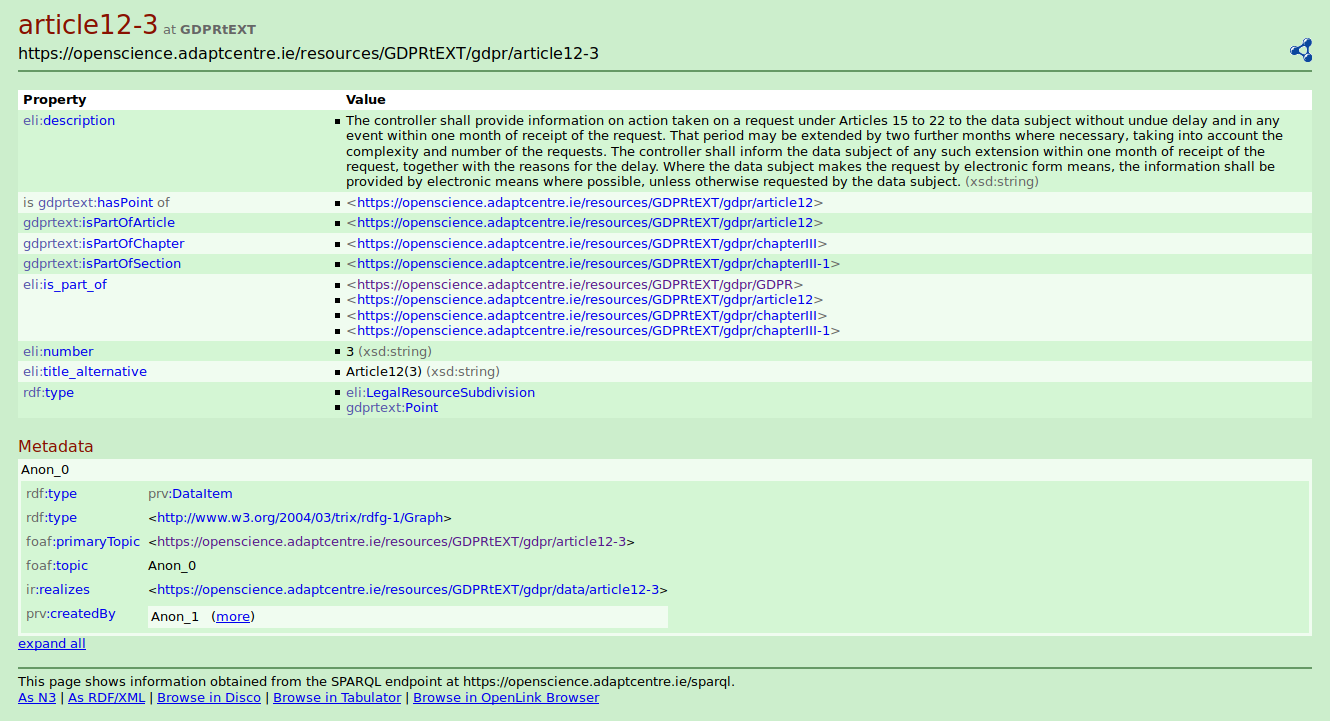
\includegraphics[width=\linewidth]{img/gdprtext-pubby}
    \caption{Article 12(3) in GDPRtEXT as RDF displayed using Pubby \cite{}}
    \label{fig:vocab:gdprtext-pubby}
\end{figure}

\subsection{Resource Description \& Application}
A visual summary of the concepts within GDPRtEXT is presented in Figures \ref{fig:vocab:gdprtext-summary-a} and \ref{fig:vocab:gdprtext-summary-b}.

\begin{figure}[htbp]
    \centering
    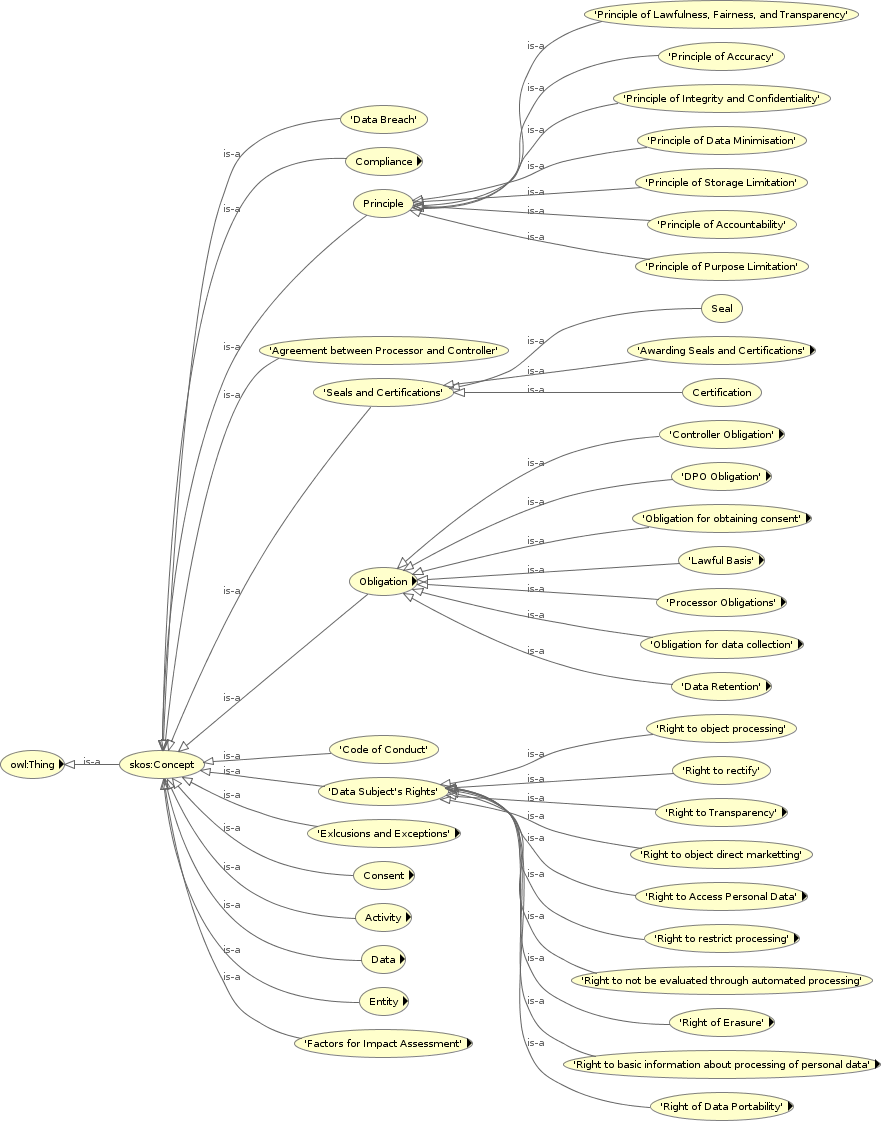
\includegraphics[width=0.75\linewidth]{img/gdprtext-summary-a}
    \caption{Visual overview of concepts in GDPRtEXT - part (a) \cite{}}
    \label{fig:vocab:gdprtext-summary-a}
\end{figure}
\begin{figure}[htbp]
    \centering
    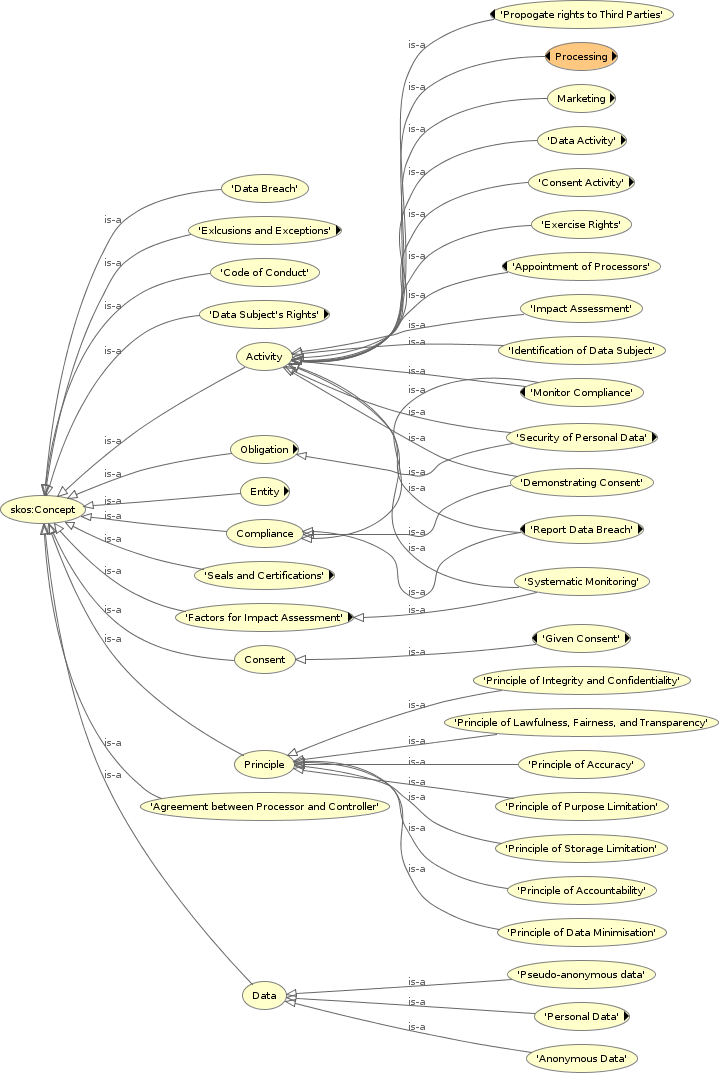
\includegraphics[width=0.75\linewidth]{img/gdprtext-summary-b}
    \caption{Visual overview of concepts in GDPRtEXT - part (b) \cite{}}
    \label{fig:vocab:gdprtext-summary-b}
\end{figure}

\subsubsection{Concepts for description structure of text}
GDPRtEXT extends the European Legislation Identifier (ELI) \cite{} ontology published by the European Publications Office with granular concepts to represent each individual clause within the GDPR. 
ELI provides the class \textit{LegalResource} to indicate a legislative document and its sub-class \textit{LegalSubResource} to indicate a component or part of that resource. GDPRtEXT extends the \textit{LegalSubResource} concept with classes Chapter, Section, Article, Point (indicates Paragraph), SubPoint (indicates Sub-Paragraph), Recital, and Citation using the sub-class mechanism.

The ELI provides properties \textit{has\_part} and its inverse \textit{is\_part\_of} to indicate connections between two legal resources. GDPRtEXT extends these to indicate hierarchical relations between chapters, sections, articles, points, and sub-points.

\subsubsection{Concepts about Data}
GDPR mentions different types of data, based on which various obligations and requirements are set forth in relation to compliance. GDPRtEXT provides the top-level concept of \textit{Data} to indicate the abstract term of `data'.

The crux of GDPR is based on personal data, which is defined in Article 4(11) and is represented by  \textit{PersonalData}, with special categories defined in Article 9(11) requiring additional obligations regarding its processing and handling, and represented by \textit{SpecialCategoryPersonalData} in GDPRtEXT. Types of special categories mentioned include criminal data, genetic data, health data, and racial data which are defined as sub-classes in GDPRtEXT.

GDPR also mentions data in the context of anonymising and pseudo-anonymising processes, with their outcomes specified using the \textit{AnonymousData} and \textit{PseudoAnonymousData} concepts.

\subsubsection{Concepts about Consent}
The top-level concept of `consent' is represented by \textit{Consent} class in GDPRtEXT with its definitions based in Articles 4(11), 6(1) and Recitals 32, 40. It is sub-classed to indicate `given consent' - which is a legal basis and is therefore a sub-class of both \textit{Consent} and \textit{LegalBasis}. \textit{GivenConsent} is further sub-classed to indicate `valid consent' which carries obligations of ensuring the consent is valid and meets the requirements of GDPR and is therefore also defined as the sub-class of \textit{ObligationForObtainingConsent}. These obligations are represented by sub-classing the \textit{ValidConsent} concept regarding conditions of - freely given, informed, specific, voluntary, and opt-in.

\subsubsection{Concepts about Entities}
\textit{Entity} represents the top-level concept of `entity' indicating any institution, company, corporation, partnership, government agency, university, or any other organization including individuals. 
It is sub-classed to indicate entities mentioned in GDPR, which are - Data Subject, Controller, Processor, Sub-Processor, Data Protection Officer (DPO), and Data Protection Authority (DPA). Additionally, relevant concepts associated with entities are also defined, which are -  Representative of Controller, Representative of Processor, Certification Body, and Regulatory Authority.

\subsubsection{Concepts about Activities}
`Activity' refers to some process or action mentioned, referred, implied, or defined by the requirements of GDPR compliance. To represent these, GDPRtEXT defines activities regarding consent and personal data processing, as well as other activities related to the functioning of the GDPR such as reporting data breach and demonstrating consent. The top-level concept `Activity' represents the abstraction of all activities, which is specialised into `ConsentActiity' and `DataActivity' to indicate involvement of consent and personal data respectively.

Consent activities defined within GDPRtEXT consist of obtaining consent and withdrawing consent. Regarding data, activities are defined to represent use, archival, collection, cross-border transfer, erasure, copying, rectifying, sharing, and storage. In these, the activity associated with usage of personal data is equivalent to its common and synonymous usage with the term `processing'. Activities for indicating context of processing include - automated processing,  automated decision making with significant effects, confirming or matching datasets, large scale processing, processing affected or vulnerable individuals, processing sensitive data, processing using untested technologies, and unlawful processing.

GDPRtEXT also provides activities associated with reporting of data breach, which include obligations and actions such as - report data breach, maintain record of breach, notify data subject of breach, report breach to controller (for processors), and report breach to DPA within 72 hours. Other activities provided are - security of personal data, appointment of processors, demonstrating consent, exercise rights, identification of data subject, impact assessment, marketing, direct marketing, monitor compliance, propagate rights to third parties, and systematic monitoring.

\subsubsection{Concepts about Compliance}
Concepts associated with compliance are provided to indicate actions or terms used in the process of maintaining, documenting, evaluating, and demonstrating compliance. The top-level concept \textit{Compliance} represents the abstract notion of compliance. Other terms derived from this include - Demonstration of Consent, Monitor Compliance, and Report Data Breach.

\subsubsection{Concepts about Principles}
GDPRtEXT represents principles using the top-level concept of \textit{Principle}, which are specialised to indicate principles associated with - Accountability; Accuracy; Data Minimisation; Integrity and Confidentiality; Lawfulness, Fairness, and Transparency; Purpose Limitation; and Storage Limitation.

\subsubsection{Concepts about Rights}
To represent rights, GDPRtEXT provides top-level concepts representing each of the rights, with further concepts associated with the rights represented as sub-classes. The right of data portability is represented by the concept \textit{RightOfDataPortability} with related concepts regarding providing copy of personal data, commonly used data format, machine readable format, structured, and supporting reuse.

The right of erasure is represented by the concept \textit{RightOfErasure} with related concepts provided regarding obligation to erase data when consent is withdrawn, or when data is no longer needed for original purpose. The right to access personal data is represented by the concept \textit{RightToAccessPersonalData} with related concepts for indicating if and where controller is processing data, whether there is automated processing with significant effects on data subject, categories of data being processed, categories of recipients data is shared with, existence of rights, information about processing, source of data, storage period, and ensuring no charges are levied for provision of rights.

The right to basic information about processing is represented by the concept \textit{RightToBasicInformationAboutProcessing} and is accompanied with its related concept regarding information about third parties. The concept \textit{RightToRestrictProcessing} represents the right to restrict processing, and is accompanied with conditions such as - accuracy is contested, data no longer needed for original purpose, and processing is unlawful. The right to transparency is represented by the concept \textit{RightToTransparency} with related concepts regarding conditions of concise, easily accessible, intelligible, and transparent. Other rights provided correspond with right to - not be evaluated through automated processing, object to direct marketing,  object to processing, and right of rectification.

\subsubsection{Concepts about Obligations}
GDPRtEXT defines concepts regarding obligations of controllers, processors, DPOs, consent, and compliant processing of personal data based on a legal basis. Obligations of controllers are represented by the concept \textit{ControllerObligation} with related concepts also provided regarding  appointment of processors, accountability, controller responsibility, co-operation with DPA, data protection by design and default, data security, liability of joint controller(s), maintaining records of processing activities, privacy by design, propagate rights to third parties, and reporting data breach.

For rights of processors, the concept \textit{ProcessorObligaion} is provided along with its related concepts for appointing sub-processors, assisting in complying with rights, compliance with controller's instructions, co-operate with DPA, data security, impose confidentiality on personnel, inform controller of conflict with law, maintain records of processing activities, only act on documented instructions, propagate rights to third parties, provide controller with information for compliance, report data breach to controller, restrictions on cross-border transfers, and return or destroy personal data at end of term.

The concept \textit{DPOObligation} represents obligations of a DPO, for which the concept \textit{MonitoringCompliance} is provided to indicate monitoring of compliance. The obligations related to lawful basis for processing are represented by \textit{LawfulBasisForProcessing} along with related concepts for contract with data subject, exempted by national law, employment law, given consent, historic, statistical, or scientific purposes, legal claims, legal obligation, legitimate interest, made public by data subject, medical, diagnostic, or treatment, not for profit org., public interest, purpose of new processing, and vital interest.

Obligations regarding valid consent are represented by \textit{ValidConsent} with related concepts to indicate that consent should be freely given, informed, specific, voluntary, and opt-in. 
Obligations for obtaining consent are represented by \textit{ObligationForObtainingConsent} and include concepts for information about third parties, indicating consent can be withdrawn easily, and conditions regarding information provided for obtaining consent such as - it should be clear, providing explanation of processing, should not be from silence or inactivity, should be demonstrable, should be distinguishable from other matters, and that is should produce valid consent.

Obligations for data collection are represented by \textit{ObligationForDataCollection}, which is accompanied with related concepts for indicating accurate collection, specification of explicit purpose, ensuring legitimate purpose, ensuring it is not further processed than original purpose, and ensuring it is limited to specified purpose.
Obligations for retention of personal data are represented by \textit{ObligationForRetentionOfPersonalData} and include related concepts about    retention of personal data, ensuring it is adequate for processing, ensuring it is identifiable for required processing, obligation to kept it up to date, ensuring it is limited for processing, obligation to rectify inaccuracies, and ensuring it is relevant for processing. 
The concept \textit{ObligationForSecurityOfPersonalData} represents the obligation regarding security of personal data, which consists of related concepts regarding accidental loss, damage, destruction, and unlawful processing.

\subsubsection{Concepts about Seals and Certifications}
GDPRtEXT provides concepts of \textit{Seal} and \textit{Certification} for representing seals and certifications as provided by GDPR to assist with the maintenance and demonstration of compliance. It also provides concepts to represent conditions for seals and certifications, represented by the concept \textit{ConditionsForSealsAndCertifications} which consist of concepts related to adherence to seal/certification, having a maximum validity of 3 years, and a voluntary system of accreditation. 

\subsubsection{Example Use-Case: Compliance Reporting}
This example use-case takes a look at how references to GDPR can aid in creation of reports which document information regarding compliance. Consider a system for creation of compliance reports that stores information related to each of the obligations it addresses from the GDPR. It uses the EARL\footnote{\url{}} vocabulary for expressing results of conformance checks within the report. GDPRtEXT is used to link the resources in EARL reports with articles and points within the GDPR as well as to express and define concepts related to compliance in a suitable and comprehensible manner. Through this, the information about compliance checks is linked and associated with the specific articles of GDPR.

EARL provides a standardized vocabulary to describe specific resources and relationships that are relevant to test reporting. The core construct of EARL is an \textit{Assertion}, which describes the context and outcome of an individual test execution. It contains the following information (copied verbatim from EARL website):

\begin{itemize}
    \item \textit{Assertor} - This can include information about who or what ran the test. For example human evaluators, automated accessibility checkers, or combinations of these.
    \item \textit{Test Subject} - This can include web content (such as web pages, videos, applets, etc.), software (such as authoring tools, user agents, etc.), or other things being tested.
    \item \textit{Test Criterion} - What are we evaluating the test subject against? This could be a specification, a set of guidelines, a test from a test suite, or some other testable statement.
    \item \textit{Test Result} - What was the outcome of the test? A test result could also include contextual information such as error messages or relevant locations within the test subject.
\end{itemize}

Taking the example of Right to Data Portability, the EARL report in Listing.\ref{listing:vocab:gdprtext-earl} represents compliance checks for conditions associated with linked articles in GDPR (Article 20). The compliance system has a module \textit{\_system\_dataportability} that checks the software that handles the provision of a copy of personal data \textit{\_org\_dataportability} through the test case \textit{\_test\_provide\_data\_copy} and generates the report which shows that the test has passed through \textit{\_result\_pass}.

\begin{lstlisting}[label={listing:vocab:gdprtext-earl},caption={Use of GDPRtEXT to link tests with GDPR Articles in EARL report}]
@prefix earl: http://www.w3.org/ns/earl# .
@prefix dct:  http://purl.org/dc/terms/ .
@prefix gdprtext: http://purl.org/adaptcentre/resources/GDPRtEXT# .

:_org_dataportability
    a    earl:TestSubject, earl:Software ;
    dct:description """System that handles data portability requests"""@en ;
    dct:title "Data Portability Handler"@en .

:_system_dataportability
    a    earl:Assertor ;
    dct:description """Module checking data portability obligations"""@en ;
    dct:hasVersion "1.4" ;
    dct:title "DataPortability Module"@en ;
    earl:asserts { :_org_dataportability :_result_pass :_test_provide_data_copy } .

:_result_pass
    a    earl:ResultProperty ;
    earl:date "2018-01-01" ;
    earl:validity earl:Pass ;
    earl:confidence earl:High .

:_test_provide_data_copy
    a    earl:TestCase ;
    earl:testMode earl:automatic ;
    dct:title "Test provision of data copy"@en ;
    dct:description """Tests whether system provides a copy of personal data on exercising right to data portability"""@en ;
    dct:subject gdprtext:article20 .
\end{lstlisting}

Now to gather such related resources together, a SPARQL query (simplified) would focus on the link between \textit{TestCase} and its result using \textit{earl:validity}, as shown in Listing.\ref{listing:vocabs:gdprtext-sparql}.
These tests can be further combined into test suites to group compliance checks related to each article or a particular concept and structure the documentation around this form of logical grouping of concepts.
In this manner, the use of GDPRtEXT to link tests and results with documentation enables automation of information retrieval and management.

\begin{lstlisting}[label={listing:vocabs:gdprtext-sparql},caption={SPARQL query and results showing retrieved GDPR test results by article}]
SELECT ?gdpr ?result ?confidence ?mode WHERE {
    ?assertor a earl:Assertor .
    ?assertor earl:asserts ?assertion .

    ?testcase rdf:predicate ?assertion .
    ?testcase a earl:TestCase .
    ?testcase dct:subject ?gdpr .
    ?testcase ear:testMode ?mode .

    ?testresult rdf:object ?assertion .
    ?testresult a earl:ResultProperty .
    ?testresult earl:validity ?result .
    ?testresult earl:confidence ?confidence .
}

| gdpr          | result     | confidence     | mode          |
|-----------    |--------    |------------    |-----------    |
| article16     | pass       | low            | automatic     |
| article17     | pass       | high           | automatic     |
| article18     | fail       | high           | manual        |
| article19     | pass       | high           | automatic     |
\end{lstlisting}

\subsubsection{Example Use-Case: Mapping between DPD and GDPR obligations}
The second application of GDPRtEXT demonstrates the linking of obligations between the GDPR and Data Protection Directive (DPD), which is the previous data protection legislation. Given that DPD was adopted in 1995, and was superseded by the GDPR in 2016, there are a large number of solutions and approaches regarding compliance with DPD that already exist and are used in practice. By linking the obligations between DPD and GDPR it is possible to investigate reuse of these existing solutions for GDPR compliance. To that end, a mapping from DPD obligations to GDPR obligations containing annotations that describe the nature of change between the two is constructed by linking the articles of DPD and GDPR.

To model the annotations as a RDF resource, a linked data version of the DPD was created similar to GDPRtEXT which assigned URIs for every resource in the legislation. This enabled referring to each individual clause in the DPD and linking it with relevant clauses in the GDPR. 
The annotations, available online\footnote{\url{https://openscience.adaptcentre.ie/projects/GDPRtEXT/dpd_mapping.html}}, are consist of references from a clause in DPD to its corresponding clause in the GDPR with an expression of change between the two. The nature of change is represented by the values of: same - indicating no change, reduced - indicating reduction of obligation, slightly changed - indicating minor change, completely changed - indicating major change, and extended - indicating addition of obligations.

To demonstrate the application of existing work regarding DPD compliance towards meeting GDPR obligations, previous existing work using XACML rules to denote DPD compliance \cite{}\cite{} were utilised to assess their suitability in meeting GDPR requirements.
For each link between DPD and GDPR obligations in the annotation, a record was also added to indicate whether the corresponding XACML rule for DPD compliance needed to be changed. The notation \textit{N/A} was used to denote the case where no XACML rules existed for a particular DPD obligation and the corresponding obligation in GDPR had changed and had additional requirements. 
% The value \textit{No} was used to indicate no changes in the GDPR obligation compared to the DPD obligation, so that the existing XACML rule would be sufficient to meet GDPR requirements. Similarly \textit{Yes} was used to indicate a change required in the XACML rule to handle the obligation.

The class \textit{DPDToGDPR\_Annotation} represents annotations between DPD and GDPR, with an example instance depicted in Listing.\ref{listing:vocabs:gdprtext-xacml}. The property \textit{resourceInDPD} is used to refer to the particular clause within DPD through its URI. Similarly, the property \textit{resourceInGDPR} is used to refer to the corresponding clause in GDPR. The nature of change is defined using the property \textit{hasChange} whose value is an instance of the class \textit{ChangeInObligation}, with defined instances for Extended, Same, Reduced, CompletelyChanged, and SlightlyChanged. Similarly, the change in the XACML rules is defined as a property whose values are one of Yes, No, and N/A defined as instances of the class \textit{ChangeInXACMLRule}. Comments are defined using the \textit{rdfs:comment} property.
\begin{lstlisting}[label={listing:vocabs:gdprtext-xacml},caption={Example annotation of associating obligation between DPD and GDPR with indication of corresponding changes required to reuse DPD compliance XACML rules for GDPR requirements}]
@prefix gdpr: https://w3id.org/GDPRtEXT/gdpr# .
@prefix dpd: https://w3id.org/GDPRtEXT/dpd# .
@prefix rdfs: http://www.w3.org/2000/01/rdf-schema# .

dpd:mappingrule6
    a dpd:DPDToGDPR_Annotation ;
    dpd:hasChange dpd:ChangeExtended ;
    dpd:hasXACMLChange dpd:XACMLNoChange ;
    dpd:resourceInDPD dpd:Article7 - a ;
    dpd:resourceInGDPR gdpr:Article6-1-a ;
    rdfs:comment "added consent given to ..." .
\end{lstlisting}


\subsection{Evaluation}
The assessment of the extent to which GDPRtEXT meets the requirements outlined in \autoref{sec:voc:gdprtext-engineering} consists of evaluating whether the ontology and dataset produced is sufficient to enable granular linking of information with the concepts and clauses of the GDPR. Based on the presented work, GDPRtEXT meets these requirements and enables answering the competency questions related to use of GDPR in the compliance process.

In terms of ontology assessment, the methodology outlined in \autoref{sec:voc:methodology} provides the criterion for evaluation of the quality of ontology as well as its documentation. GDPRtEXT fulfils these, based on tests undertaken using the OOPS! tool and by following the best practices community guidelines for ontology documentation.
The publication of GDPRtEXT in Irish open data portal demonstrates the quality of the work, based on the 5 star rating given to it as a linked open dataset.

GDPRtEXT, and the work described in this section, was published in the resource track at Extended Semantic Web Conference \cite{}. The publication described the creation of the resource, summarised its contents, and also provided mapping of DPD obligations with GDPR using a linked data approach and XACML to denote which obligations from DPD could be re-used towards GDPR compliance. Through this, the research and developed resources were peer-reviewed and adopted.
Further validation is provided through a survey of legal approaches and works in the state of the art \cite{} which includes GDPRtEXT as one of the resources surveyed and demonstrates that GDPRtEXT is unique in its provision of GDPR as a machine-readable resource.

\subsection*{Summary}
The GDPRtEXT resource represents the first major contribution of this thesis. It provides a linked data version of the text of GDPR and a vocabulary of its concepts, and fulfils research objectives $RO3(a)$ and $RO5(b)$ - as outlined in \autoref{sec:intro:RQ}. It enables exposing each individual article or point within the GDPR as a unique resource through URIs provided using semantic web notations.
GDPRtEXT thus enables machine-readable links to be established between information and the text of GDPR as well as concepts pertaining to its compliance.

The use of GDPRtEXT makes it possible to create approaches that automate the generation and querying of information associated with GDPR - such as for compliance, management of business processes, or generation of privacy policies. The compatibility offered by use of ELI ontology ensures alignment with official documents produced by the European Publications Office in the future.
Finally, GDPRtEXT fills an important gap in the state of the art regarding machine-readable approaches for linking information with legal text.
GDPRtEXT has been released as an open resource under the permissive CC-by-4.0 license. It has been published in Zenodo, Datahub, and has been incorporated into Ireland’s open data portal as a 5-star linked open dataset.

% GDPRov
\section{GDPRov - Ontology for GDPR activities associated with Personal Data and Consent}\label{sec:voc:GDPRov}

aim/objective: provide representations of activities in ex-ante and ex-post phases associated with processing of personal data and consent for GDPR compliance

\subsection{Requirements Gathering \& Ontology Engineering}

* identify activities using analysis in Ch 4 and  background in Ch 2; use compliance questions in Ch4 as comptency questions
* identfiy suitable represenations of ex-ante and ex-post activities --> PROV-O and P-Plan
* formulate ontological representations

\subsection{Ontology Description \& Application}

* copy from paper

\subsection{Evaluation}

* adherence to CQ
* compare against sota
* peer reviewed publication

\subsection*{Summary}

% GConsent
\section{GConsent - Ontology for Consent Information for GDPR Compliance}\label{sec:voc:GConsent}

aim/objective: representation of contextual information about consent according to requirements of GDPR compliance

* inform that GDPRov is not sufficient to evaluate consent compliance

\subsection{Requirements Gathering \& Ontology Engineering}

* identfiy information required for compliance - ch2 background
* use analysis in ch 4 and ch 2 background
* use compliance questions in ch 4 as competency questions
* semi-formal consultation with legal expert (law prof. TCD)

\subsection{Ontology Description \& Application}

* copy from paper

\subsection{Evaluation}

* CQ, use-cases
* compare against SotA
* peer-reviewed publication

\subsection*{Summary}

* only vocab in sota
* further work ongoing to combine with CR standard to adopt GDPR and other emerging laws
* ??? to mention ??? consultaition with research Mastercard on semantic representation of consent

% DPV
\section{Data Privacy Vocabulary (DPV)}\label{sec:voc:DPV}

* intro as to why this is relevant
* What is the DPVCG
* What is DPV
* My role

\subsection{W3C Data Privacy Vocabularies and Controls CG}
* What is the CG
* Aims, objectives, how it started, when, SPECIAL
* members???
* cite SW4SG paper

\subsection{Description of Data Privacy Vocabulary}
* copy from ODBASE paper

\subsection{Comparison with GDPRtEXT, GDPRov, GConsent, and SotA}

\subsection*{Summary}

\section{Chapter Summary}